\documentclass[10pt]{beamer}
\usepackage{adjustbox}
\usepackage{amsmath}
\usepackage{graphicx}
\usepackage{float}
\usepackage{caption}
\usepackage{listings}
\usepackage{xcolor}
\usepackage{multimedia}
\usepackage[backend=biber,style=alphabetic]{biblatex} % Bibliography management
\addbibresource{references.bib}
\graphicspath{{tex/}}
\colorlet{punct}{red!60!black}
\definecolor{background}{RGB}{240, 248, 255}
\definecolor{delim}{RGB}{20,105,176}
\colorlet{numb}{magenta!60!black}

\lstdefinelanguage{json}{
  basicstyle=\ttfamily\footnotesize\color{black},
  numbers=left,
  numberstyle=\scriptsize,
  stepnumber=1,
  numbersep=8pt,
  showstringspaces=false,
  breaklines=true,
  frame=lines,
  backgroundcolor=\color{background},
  literate=
  *{0}{{{\color{numb}0}}}{1}
  {1}{{{\color{numb}1}}}{1}
  {2}{{{\color{numb}2}}}{1}
  {3}{{{\color{numb}3}}}{1}
  {4}{{{\color{numb}4}}}{1}
  {5}{{{\color{numb}5}}}{1}
  {6}{{{\color{numb}6}}}{1}
  {7}{{{\color{numb}7}}}{1}
  {8}{{{\color{numb}8}}}{1}
  {9}{{{\color{numb}9}}}{1}
  {:}{{{\color{punct}{:}}}}{1}
  {,}{{{\color{punct}{,}}}}{1}
  {\{}{{{\color{delim}{\{}}}}{1}
  {\}}{{{\color{delim}{\}}}}}{1}
  {[}{{{\color{delim}{[}}}}{1}
  {]}{{{\color{delim}{]}}}}{1},
}

\lstset{frame=single, showstringspaces=false, columns=fixed, basicstyle={\ttfamily}, commentstyle={\it}, numbers=left, tabsize=4}

\definecolor{codebackground}{RGB}{240, 248, 255}
\definecolor{codecomment}{RGB}{106,153,85}
\definecolor{codekeyword}{RGB}{30,30,255}
\definecolor{codestring}{RGB}{163,21,21}
\definecolor{codenumber}{RGB}{100,100,100}

\lstdefinestyle{modernstyle}{
  backgroundcolor=\color{codebackground},
  commentstyle=\color{codecomment},
  keywordstyle=\color{codekeyword},
  numberstyle=\tiny\color{codenumber},
  stringstyle=\color{codestring},
  basicstyle=\ttfamily\footnotesize\color{black},
  breakatwhitespace=false,
  breaklines=true,
  captionpos=b,
  keepspaces=true,
  numbers=left,
  numbersep=5pt,
  showspaces=false,
  showstringspaces=false,
  showtabs=false,
  tabsize=4
}

\lstset{style=modernstyle}

\usetheme{Copenhagen}
\usecolortheme{default}
\setbeamertemplate{navigation symbols}{}
\setbeamertemplate{page number in head/foot}[totalframenumber]

\title[Projet M2 Incertitude]{
  
\includegraphics[width=0.8\textwidth]{images/logo-ufr.png}\\
  Projet M2 d'Incertitude:\\
Modélisation d'un flux routier}
\author[PA Senger]{Pierre-Antoine SENGER}
\date{}

\begin{document}

% \begin{frame}[plain]
%     \begin{center}
%     \begin{tabular}{c c c}
%     \includegraphics[width=100px]{images/logo-irma.png} &
%     \includegraphics[width=100px]{images/logo-inria.png} &
%     \includegraphics[width=100px]{images/logo-hidalgo2.png} \\
%     
\includegraphics[width=100px]{images/logo-ufr.png} &
%     \includegraphics[width=100px]{images/logo-cemosis.png} &
%     \includegraphics[width=100px]{images/logo-numpex.png} \\
%     \end{tabular}
%     \end{center}
% \end{frame}

\begin{frame}{}
  \titlepage
\end{frame}

\begin{frame}{Context}
  \textcolor{blue}{Equation de Burgers:}
  $$ \partial_t \rho + \partial_x (\rho v(\rho)) = 0 $$
  \begin{itemize}
    \item $\rho$ : \textbf{densité} de véhicules
    \item $v(\rho) = v_{max} (1 - \frac{\rho}{\rho_{max}})$ : \textbf{vitesse} des véhicules
  \end{itemize}

  \textcolor{blue}{Condition initial (problème de Riemann):}
  $$ \rho(0, x) =
  \begin{cases} r_{in} & \text{,si } x < x_C \\
    r_{out} & \text{,si } x \geq x_C
  \end{cases} $$
  \begin{itemize}
    \item $r_{in}$ : \textbf{densité} de véhicules à \textbf{gauche} de $x_C$
    \item $r_{out}$ : \textbf{densité} de véhicules à \textbf{droite} de $x_C$
    \item $x_C$ : position de la \textbf{discontinuité}
  \end{itemize}

\end{frame}

\begin{frame}{Décongestion}
  $r_{in} > r_{out}$ \\
  \begin{figure}
    \centering
    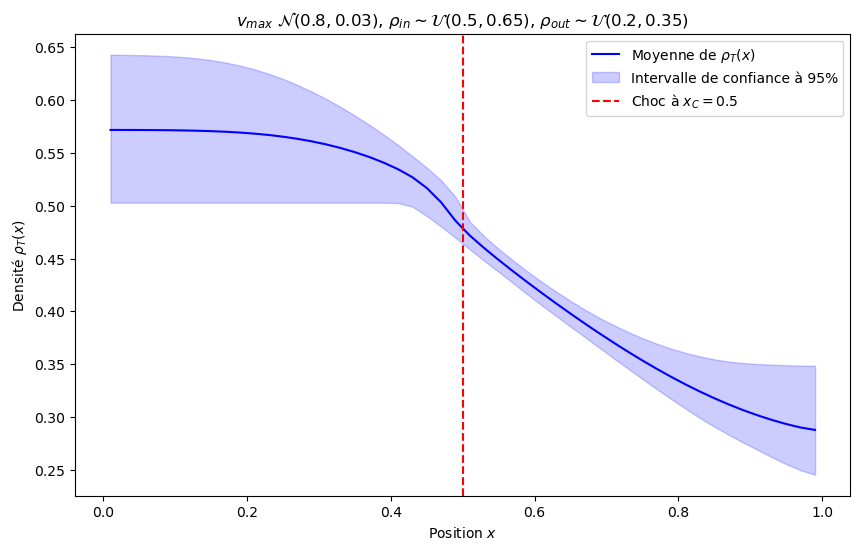
\includegraphics[width=0.8\textwidth]{images/rin_greater_rout.png}
    \caption{Décongestion}
  \end{figure}
\end{frame}

\begin{frame}{Bouchon}
  $r_{in} < r_{out}$ \\
  \begin{figure}
    \centering
    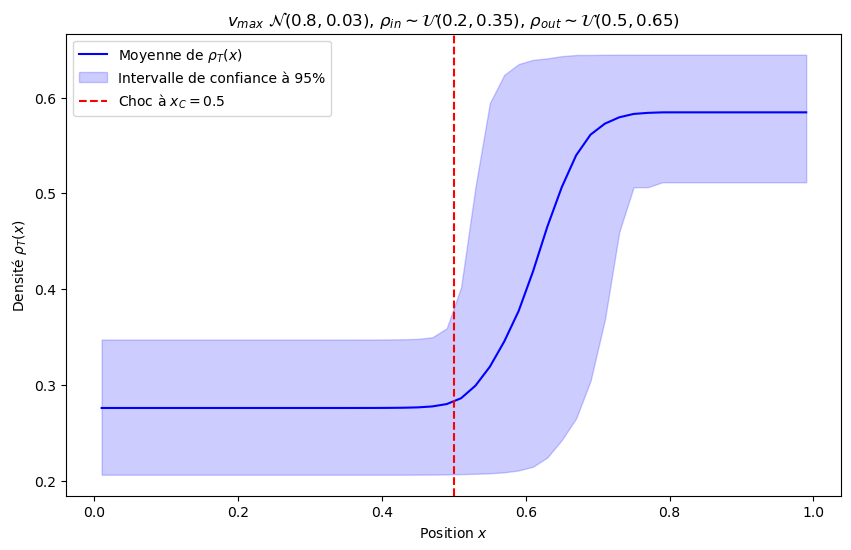
\includegraphics[width=0.8\textwidth]{images/rin_less_rout.png}
    \caption{Formation d'un bouchon}
  \end{figure}
\end{frame}

\begin{frame}{Objectifs}
  \begin{itemize}
    \item Est-ce que le bouchon se forme ?
    \item Est-ce que le bouchon se dissipe ?
    \item Quel est le temps de dissipation du bouchon ? Sur quels critères ?
    \item Quelles sont les variables qui influes le plus sur le temps de dissipation ?
  \end{itemize}
\end{frame}

\begin{frame}{Critères de formation}
  \begin{figure}
    \centering
    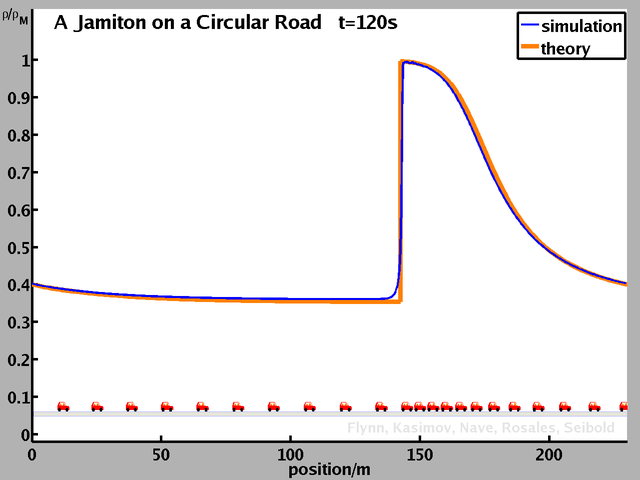
\includegraphics[width=0.8\textwidth]{images/traffic_jam_mit.png}
    \caption{Formation d'un bouchon \cite{trafficJamMIT}}
  \end{figure}
\end{frame}

\begin{frame}{Temps de dissipation}
  \begin{figure}
    \centering
    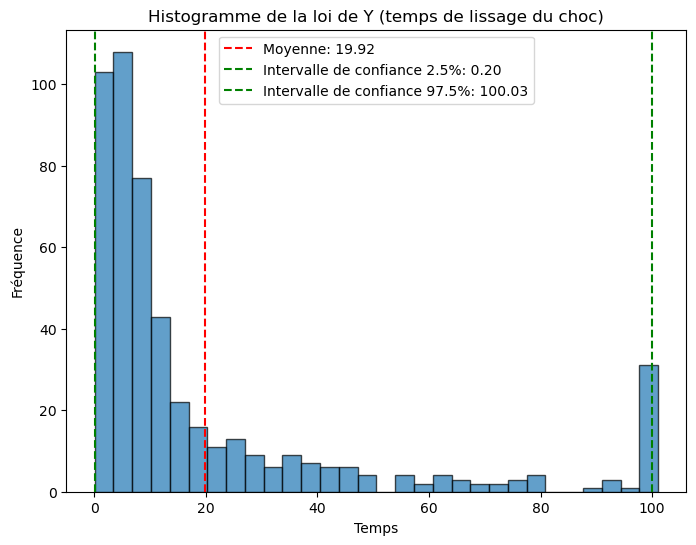
\includegraphics[width=0.8\textwidth]{images/loi_de_Y.png}
    \caption{Loi de Y via une simulation Monte-Carlo}
  \end{figure}
\end{frame}

\begin{frame}{Indices de Sobol (1)}
  \begin{figure}
    \centering
    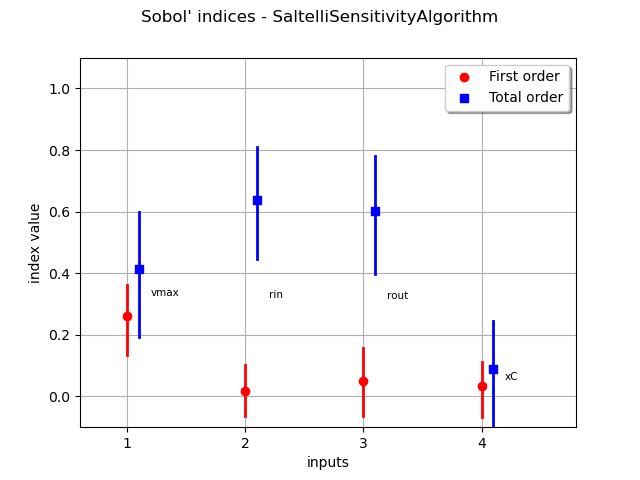
\includegraphics[width=0.8\textwidth]{images/sobol1.png}
    \caption{Indices de Sobol via une simulation Monte-Carlo (OpenTURNS\cite{baudinOpenTURNSIndustrialSoftware2016})}
  \end{figure}
\end{frame}

\begin{frame}{Indices de Sobol (2)}
  \begin{figure}
    \centering
    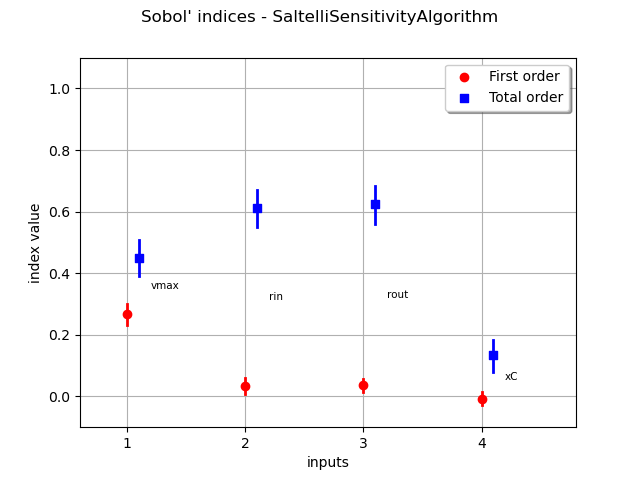
\includegraphics[width=0.8\textwidth]{images/sobol2.png}
    \caption{Indices de Sobol via un metamodel (MLP)}
  \end{figure}
\end{frame}

\begin{frame}{Indices de Shapley}
  \begin{figure}
    \centering
    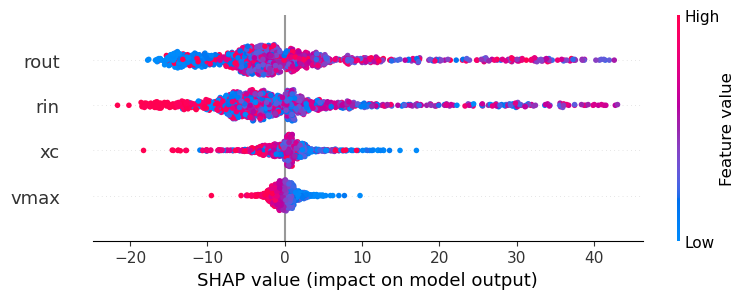
\includegraphics[width=0.8\textwidth]{images/shapley.png}
    \caption{Indices de Shapley via un metamodel MLP (SHAP\cite{SHAP})}
  \end{figure}
\end{frame}

\begin{frame}{The end}
  \Large
  \centering
  \textbf{Thank you for your attention!} \\
  \vspace{1em}
  
\includegraphics[height=1cm]{images/party-emoji.png} \\
  \vspace{1em}
  \textbf{Any questions?} \\
  \vspace{2em}
  \small
  \textit{Contact Information:} \\
  pierre.antoine.senger@gmail.com \\
  github.com/PA-Senger
\end{frame}

\begin{frame}{References}
  \printbibliography
\end{frame}

\end{document}